\section{Amarinda Damar}\label{amarinda-damar}

Tags: NPC Creatore: Lorenzo Luogo: Disharta, Goldendoor

\section{\texorpdfstring{\textbf{Amarinda
Damar}}{Amarinda Damar}}\label{amarinda-damar-1}

\begin{center}\rule{0.5\linewidth}{0.5pt}\end{center}

\begin{figure}
\centering
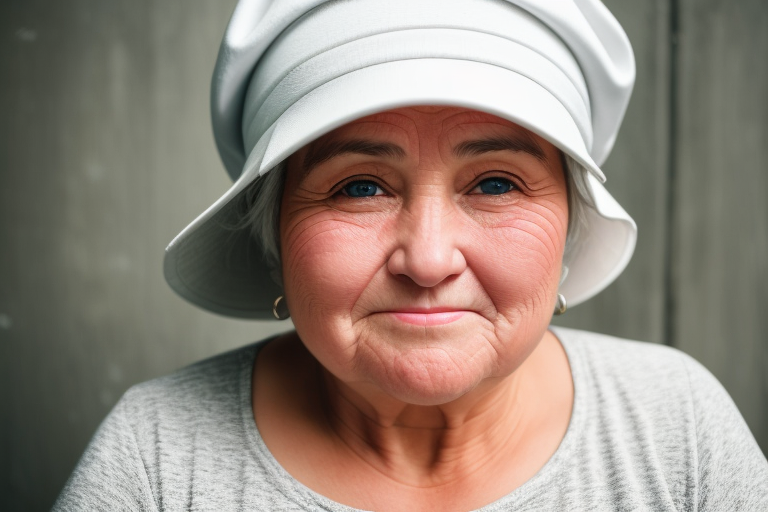
\includegraphics{03_AMARINDA.png}
\caption{03\_AMARINDA.png}
\end{figure}

Informazioni Generali

Età: 75

Data di nascita: 1949

Luogo di nascita:Disharta

Razza: Umana

Classe:

Alleati:

Nemesi:

Alias:

Professione: Balia di corte

\begin{center}\rule{0.5\linewidth}{0.5pt}\end{center}

\subsection{1. Descrizione Generale}\label{descrizione-generale}

\begin{center}\rule{0.5\linewidth}{0.5pt}\end{center}

Amarinda è una donna matura con i capelli grigi e un portamento
dignitoso. Indossa abiti semplici ma ben curati, in linea con la sua
posizione nella corte reale.

\subsection{2. Biografia}\label{biografia}

\begin{center}\rule{0.5\linewidth}{0.5pt}\end{center}

Amarinda ha dedicato la maggior parte della sua vita al servizio della
famiglia reale di Disharta. È entrata al servizio della corte come
giovane dama di compagnia, ma nel corso degli anni è diventata la balia
di Leona, la principessa ereditaria dell'Impero. Nonostante non abbia
legami di sangue con la famiglia reale, il suo amore per Leona è così
profondo che la considera come una figlia.

\subsection{3. Carriera}\label{carriera}

\begin{center}\rule{0.5\linewidth}{0.5pt}\end{center}

Ha avuto il compito di prendersi cura della principessa fin dalla sua
nascita e di assicurarsi che crescesse con valori morali e principi
solidi. È stata una presenza costante nella vita di Leona, fungendo da
confidente e guida.

\subsection{4. Personalità}\label{personalituxe0}

\begin{center}\rule{0.5\linewidth}{0.5pt}\end{center}

Amarinda è una donna di grande determinazione e lealtà. È astuta e
intelligente, capace di affrontare situazioni complesse con calma e
saggezza. La sua principale preoccupazione è il benessere di Leona, e
farebbe qualsiasi cosa per proteggerla. Nonostante la sua posizione
nella corte reale, Amarinda preferisce rimanere sullo sfondo, ma il suo
affetto e il suo sostegno sono inestimabili per la principessa. Negli
ultimi tempi, ha segretamente aiutato Leona a prepararsi per la fuga,
pur negando qualsiasi coinvolgimento quando è stata interrogata dai
membri della corte. Il suo amore per la principessa l'ha spinta a
sostenere la decisione di Leona di sfidare le convenzioni imperiali e
cercare un destino diverso da quello imposto dalla corte reale.

\subsection{A. Coinvolgimenti in Eventi
Recenti}\label{a.-coinvolgimenti-in-eventi-recenti}

\begin{center}\rule{0.5\linewidth}{0.5pt}\end{center}

\href{Untitled\%20Database\%20ebdcd210a5d74a8e8603c3356a0daf65.csv}{Untitled
Database}

\subsection{B. Aggiornamenti}\label{b.-aggiornamenti}

\begin{center}\rule{0.5\linewidth}{0.5pt}\end{center}

\href{Untitled\%20Database\%20c4aa259cbb3945d5a85eef6558b6cd30.csv}{Untitled
Database}
